% ====================================================================
%  徐森林、薛春华《数学分析》（第一册）
%  \S3.2  高阶导数、参变量函数的导数、导数的 Leibniz 公式
%  源：原书印刷页 171-185（PDF 物理页 177-191）
%  底本：PaddleOCR-VL-1.6 + 高清影印比对校订
%  规范：全西文半角标点；单一落盘出口 _texout.py
% ====================================================================
\section{高阶导数、参变量函数的导数、导数的 Leibniz 公式}\label{sec:3.2}

例~\ref{ex:3.1.15} 指出, 加速度就是位移对时间 $t$ 的 2 阶导数. 自然会想到要进一步研究高阶导数.

\begin{definition}\label{def:3.2.1}
如果 $f$ 的导函数 $f'$ 在点 $x_0$ 处可导, 则称 $f'$ 在点 $x_0$ 处的导数为 $f$ 在点 $x_0$ 的 2 阶导数, 记作
\[
f''(x_0) = \lim_{x\to x_0}\frac{f'(x) - f'(x_0)}{x - x_0} = \lim_{\Delta x\to0}\frac{f'(x_0+\Delta x) - f'(x_0)}{\Delta x}.
\]
同时称 $f$ 在点 $x_0$ 处 2 阶可导. 2 阶导数也可记为 $\left.\frac{\mathrm{d}^{2}f}{\mathrm{d}x^{2}}\right|_{x=x_0}$, $\left.\frac{\mathrm{d}^{2}y}{\mathrm{d}x^{2}}\right|_{x=x_0}$.

类似可定义 3 阶, 4 阶, $\cdots$, $n$ 阶导数:
\[
\begin{aligned}
f^{(n)}(x_0) &= \lim_{x\to x_0}\frac{f^{(n-1)}(x) - f^{(n-1)}(x_0)}{x - x_0}\\
&= \lim_{\Delta x\to0}\frac{f^{(n-1)}(x_0+\Delta x) - f^{(n-1)}(x_0)}{\Delta x},
\end{aligned}
\]
$f'' = (f')'$, $f^{(4)} = (f''')'$, $\cdots$, $f^{(n)} = (f^{(n-1)})'$. $n$ 阶导数也可记为 $\left.\frac{\mathrm{d}^{n}f}{\mathrm{d}x^{n}}\right|_{x=x_0}$, $\left.\frac{\mathrm{d}^{n}y}{\mathrm{d}x^{n}}\right|_{x=x_0}$.

$f$ 在开区间 $(a,b)$ 的每一点处 $n$ 阶可导, 则称 $f$ 在 $(a,b)$ 上 $n$ 阶可导.
\end{definition}

由 $n$ 阶导数定义, 显然有
\[
(f \pm g)^{(n)} = f^{(n)} \pm g^{(n)},\quad (\lambda f)^{(n)} = \lambda f^{(n)},\ \lambda \in \mathbb{R}.
\]

\begin{theorem}[Leibniz]\label{thm:3.2.1}
设 $f$ 与 $g$ 在区间 $I$ 上都 $n$ 阶可导, 则
\[
(fg)^{(n)} = \sum_{k=0}^{n}\mathrm{C}_{n}^{k}f^{(n-k)}g^{(k)},
\]
其中, $\mathrm{C}_{n}^{k} = \frac{n!}{k!(n-k)!}$ 为组合数, $g^{(0)} = g$, $f^{(0)} = f$.
\end{theorem}

\begin{proof}
用归纳法. 当 $n = 1$ 时,
\[
(fg)' = f'g + fg' = \sum_{k=0}^{1}\mathrm{C}_{1}^{k}f^{(1-k)}g^{(k)}.
\]
假设 $n = l$ 时, 有
\[
(fg)^{(l)} = \sum_{k=0}^{l}\mathrm{C}_{l}^{k}f^{(l-k)}g^{(k)}.
\]
那么, 当 $n = l+1$ 时, 有
\[
\begin{aligned}
(fg)^{(l+1)} &= ((fg)^{(l)})' = \left(\sum_{k=0}^{l}\mathrm{C}_{l}^{k}f^{(l-k)}g^{(k)}\right)'\\
&= \sum_{k=0}^{l}\mathrm{C}_{l}^{k}\left[(f^{(l-k)})'g^{(k)} + f^{(l-k)}(g^{(k)})'\right]\\
&= \sum_{k=0}^{l}\mathrm{C}_{l}^{k}\left[f^{(l+1-k)}g^{(k)} + f^{(l-k)}g^{(k+1)}\right]\\
&= \mathrm{C}_{l}^{0}f^{(l+1)}g + \sum_{k=1}^{l}\mathrm{C}_{l}^{k}f^{(l+1-k)}g^{(k)} + \sum_{k=0}^{l-1}\mathrm{C}_{l}^{k}f^{(l-k)}g^{(k+1)} + \mathrm{C}_{l}^{l}fg^{(l+1)}\\
&= \mathrm{C}_{l+1}^{0}f^{(l+1)}g + \sum_{k=1}^{l}(\mathrm{C}_{l}^{k} + \mathrm{C}_{l}^{k-1})f^{(l+1-k)}g^{(k)} + \mathrm{C}_{l+1}^{l+1}fg^{(l+1)}\\
&= \sum_{k=0}^{l+1}\mathrm{C}_{l+1}^{k}f^{(l+1-k)}g^{(k)}.
\end{aligned}
\]
\end{proof}

\begin{example}\label{ex:3.2.1}
求 $y = x^{n}$ 的各阶导函数, $n \in \mathbb{N}$.
\end{example}

\begin{solution}
\[
\begin{aligned}
y' &= nx^{n-1},\\
y'' &= n(n-1)x^{n-2},\\
&\cdots\\
y^{(n-1)} &= n(n-1)\cdots2x,\\
y^{(n)} &= n!,\\
y^{(n+1)} &= y^{(n+2)} = \cdots = 0.
\end{aligned}
\]
\end{solution}

\begin{example}\label{ex:3.2.2}
求下列函数的各阶导函数:
(1) $y = a^{x}$ ($a > 0$), 特别地, $y = \mathrm{e}^{x}$; (2) $y = \mathrm{e}^{ax}$;
(3) $y = \sin x$; (4) $y = \cos x$; (5) $y = \frac{1}{x-a}$; (6) $y = \frac{1}{x^{2}-3x+2}$.
\end{example}

\begin{solution}
(1) $y' = a^{x}\ln a$, $\cdots$, $y^{(n)} = a^{x}(\ln a)^{n}$. 特别地, $\left(\mathrm{e}^{x}\right)^{(n)} = \mathrm{e}^{x}$.

(2) $y' = a\mathrm{e}^{ax}$, $\cdots$, $y^{(n)} = a^{n}\mathrm{e}^{ax}$.

(3) $y' = \cos x = \sin\left(x + \frac{\pi}{2}\right)$. 设 $y^{(k)} = \sin\left(x + \frac{k\pi}{2}\right)$, 则有
\[
y^{(k+1)} = (y^{(k)})' = \cos\left(x + \frac{k\pi}{2}\right)\cdot1 = \sin\left[x + \frac{(k+1)\pi}{2}\right].
\]
于是, $\forall n \in \mathbb{N}$, 有
\[
y^{(n)} = \sin\left(x + \frac{n\pi}{2}\right).
\]

(4) 类似 (3), 可证 $(\cos x)^{(n)} = \cos\left(x + \frac{n\pi}{2}\right)$, $n \in \mathbb{N}$. 或者
\[
\begin{aligned}
(\cos x)^{(n)} &= \left(\sin\left(x + \frac{\pi}{2}\right)\right)^{(n)} = \sin\left(x + \frac{\pi}{2} + \frac{n\pi}{2}\right)\\
&= \cos\left(x + \frac{n\pi}{2}\right).
\end{aligned}
\]

(5) $y = \frac{1}{x-a} = (x-a)^{-1}$,
\[
y' = -(x-a)^{-2},\quad y'' = 2(x-a)^{-3},\quad \cdots,
\]
\[
y^{(n)} = (-1)^{n}\cdot n!(x-a)^{-(n+1)} = \frac{(-1)^{n}\cdot n!}{(x-a)^{(n+1)}}.
\]

(6)
\[
\begin{aligned}
y &= \frac{1}{x^{2}-3x+2} = \frac{1}{x-2} - \frac{1}{x-1},\\
y^{(n)} &= \left(\frac{1}{x-2}\right)^{(n)} - \left(\frac{1}{x-1}\right)^{(n)} = \frac{(-1)^{n}n!}{(x-2)^{n+1}} - \frac{(-1)^{n}n!}{(x-1)^{n+1}}\\
&= (-1)^{n}n!\left[\frac{1}{(x-2)^{n+1}} - \frac{1}{(x-1)^{n+1}}\right].
\end{aligned}
\]
\end{solution}

\begin{example}\label{ex:3.2.3}
设 $f(x) = a_{n}(x-x_0)^{n} + a_{n-1}(x-x_0)^{n-1} + \cdots + a_{1}(x-x_0) + a_{0}$ 为 $n$ 次多项式, 其中 $a_{n} \neq 0$,
\[
a_{k} = \frac{f^{(k)}(x_0)}{k!},\quad k = 0, 1, \cdots, n,
\]
因此,
\[
f(x) = \sum_{k=0}^{n}a_{k}(x-x_0)^{k} = \sum_{k=0}^{n}\frac{f^{(k)}(x_0)}{k!}(x-x_0)^{k}.
\]
\end{example}

\begin{proof}
因为
\[
\begin{aligned}
f(x) &= \sum_{k=0}^{n}a_{k}(x-x_0)^{k},\\
f'(x) &= \sum_{k=1}^{n}ka_{k}(x-x_0)^{k-1},\\
&\cdots\\
f^{(l)}(x) &= \sum_{k=l}^{n}k(k-1)\cdots(k-l+1)a_{k}(x-x_0)^{k-l},\\
&\cdots\\
f^{(n)}(x) &= n!a_{n},
\end{aligned}
\]
所以, $f(x_0) = a_0$, $f'(x_0) = a_1$, $\cdots$, $f^{(l)}(x_0) = l!a_l$, $\cdots$, $f^{(n)}(x_0) = n!a_n$, 即
\[
a_{l} = \frac{f^{(l)}(x_0)}{l!},\quad l = 0, 1, \cdots, n.
\]
\end{proof}

\begin{example}\label{ex:3.2.4}
设 $y = \mathrm{e}^{x}\cos x$, 求 $y^{(n)}$, $y^{(5)}$.
\end{example}

\begin{solution}
因为 $(\mathrm{e}^{x})^{(k)} = \mathrm{e}^{x}$, $(\cos x)^{(k)} = \cos\left(x + \frac{k\pi}{2}\right)$, 故由 Leibniz 求导公式知
\[
\begin{aligned}
y^{(n)} &= \left(\mathrm{e}^{x}\cos x\right)^{(n)} = \sum_{k=0}^{n}\mathrm{C}_{n}^{k}\left(\mathrm{e}^{x}\right)^{(n-k)}\left(\cos x\right)^{(k)}\\
&= \sum_{k=0}^{n}\mathrm{C}_{n}^{k}\mathrm{e}^{x}\cos\left(x + \frac{k\pi}{2}\right),
\end{aligned}
\]
当 $n = 5$ 时,
\[
\begin{aligned}
y^{(5)} &= \sum_{k=0}^{5}\mathrm{C}_{5}^{k}\mathrm{e}^{x}\cos\left(x + \frac{k\pi}{2}\right)\\
&= \mathrm{e}^{x}\left[\cos x + 5\cos\left(x + \frac{\pi}{2}\right) + 10\cos\left(x + \frac{2\pi}{2}\right) + 10\cos\left(x + \frac{3\pi}{2}\right)\right.\\
&\quad \left. + 5\cos\left(x + \frac{4\pi}{2}\right) + \cos\left(x + \frac{5\pi}{2}\right)\right]\\
&= \mathrm{e}^{x}(\cos x - 5\sin x - 10\cos x + 10\sin x + 5\cos x - \sin x)\\
&= 4\mathrm{e}^{x}(\sin x - \cos x).
\end{aligned}
\]
\end{solution}

\begin{example}\label{ex:3.2.5}
设 $y = x^{2}\cos x$, 求 $y^{(50)}$.
\end{example}

\begin{solution}
由 Leibniz 求导公式知,
\[
\begin{aligned}
y^{(50)} &= \sum_{k=0}^{50}\mathrm{C}_{50}^{k}\left(\cos x\right)^{(50-k)}\left(x^{2}\right)^{(k)}\\
&= x^{2}\left(\cos x\right)^{(50)} + \mathrm{C}_{50}^{1}\cdot2x\left(\cos x\right)^{(49)} + \mathrm{C}_{50}^{2}\cdot2\left(\cos x\right)^{(48)}\\
&= x^{2}\cos\left(x + \frac{50\pi}{2}\right) + 100x\cos\left(x + \frac{49\pi}{2}\right) + 2450\cos\left(x + \frac{48\pi}{2}\right)\\
&= -x^{2}\cos x - 100x\sin x + 2450\cos x\\
&= (2450 - x^{2})\cos x - 100x\sin x.
\end{aligned}
\]
\end{solution}

\begin{example}\label{ex:3.2.6}
设
\[
f(x) = \begin{cases}x^{4}\sin\frac{1}{x}, & x \neq 0,\\ 0, & x = 0,\end{cases}
\]
求 $f''(x)$.
\end{example}

\begin{solution}
由
\[
f'(0) = \lim_{x\to0}\frac{f(x) - f(0)}{x - 0} = \lim_{x\to0}\frac{x^{4}\sin\frac{1}{x} - 0}{x - 0} = \lim_{x\to0}x^{3}\sin\frac{1}{x} = 0,
\]
得到
\[
f'(x) = \begin{cases}4x^{3}\sin\frac{1}{x} - x^{2}\cos\frac{1}{x}, & x \neq 0,\\ 0, & x = 0.\end{cases}
\]
按照 2 阶导数定义, 有
\[
\begin{aligned}
f''(0) &= \lim_{x\to0}\frac{f'(x) - f'(0)}{x - 0} = \lim_{x\to0}\frac{4x^{3}\sin\frac{1}{x} - x^{2}\cos\frac{1}{x} - 0}{x - 0}\\
&= \lim_{x\to0}\left(4x^{2}\sin\frac{1}{x} - x\cos\frac{1}{x}\right) = 0,
\end{aligned}
\]
从而
\[
\begin{aligned}
f''(x) &= \begin{cases}12x^{2}\sin\frac{1}{x} - 4x\cos\frac{1}{x} - 2x\cos\frac{1}{x} - \sin\frac{1}{x}, & x \neq 0,\\ 0, & x = 0\end{cases}\\
&= \begin{cases}(12x^{2} - 1)\sin\frac{1}{x} - 6x\cos\frac{1}{x}, & x \neq 0,\\ 0, & x = 0.\end{cases}
\end{aligned}
\]
进一步, 由于极限
\[
\lim_{x\to0}\frac{(12x^{2} - 1)\sin\frac{1}{x} - 6x\cos\frac{1}{x} - 0}{x - 0} = \lim_{x\to0}\left[12x\sin\frac{1}{x} - \frac{\sin\frac{1}{x} + 6x\cos\frac{1}{x}}{x}\right]
\]
不存在, 故 $\forall n \in \mathbb{N}$, $f^{(n)}(x)$ 对 $x \neq 0$ 都是存在的, 但是 $f'''(0)$ 已不存在.
\end{solution}

\begin{definition}\label{def:3.2.2}
设函数 $f$ 在 $U \subsetneq \mathbb{R}$ 上连续, 则称 $f$ 在 $U$ 上是 $C^{0}$ 的, 记 $U$ 上 $C^{0}$ 函数的全体为 $C^{0}(U, \mathbb{R})$; 设 $r \in \mathbb{N}$, 如果 $f$ 在开集 $U \subsetneq \mathbb{R}$ 上 $r$ 阶连续可导, 则称 $f$ 在 $U$ 上是 $C^{r}$ 的, 记 $U$ 上 $C^{r}$ 函数的全体为 $C^{r}(U, \mathbb{R})$; 如果 $f$ 在开集 $U \subsetneq \mathbb{R}$ 上各阶连续可导, 则称 $f$ 在 $U$ 上是 $C^{\infty}$ 的, 记 $U$ 上 $C^{\infty}$ 函数的全体为 $C^{\infty}(U, \mathbb{R})$; 如果 $f$ 在开集 $U \subsetneq \mathbb{R}$ 上, 每一点 $x_0 \in U$ 的邻近可展开为收敛的幂级数
\[
f(x) = \sum_{n=0}^{\infty}a_{n}(x-x_0)^{n},\quad x \in (x_0 - \delta_{x_0}, x_0 + \delta_{x_0}) \subset U,
\]
则称 $f$ 在 $U$ 上是 $C^{\omega}$ 的或实解析的. 第 3 册将证明 $a_{n} = \frac{f^{(n)}(x_0)}{n!}$, 称为 $f$ 的 Taylor 系数.

记 $U$ 上 $C^{\omega}$ 函数的全体为 $C^{\omega}(U, \mathbb{R})$.
\end{definition}

\begin{example}\label{ex:3.2.7}
(1) 设 $r = 0, 1, 2, \cdots$, 则
\[
f(x) = \begin{cases}x^{2r+1}\sin\frac{1}{x}, & x \neq 0,\\ 0, & x = 0\end{cases}
\]
在 $\mathbb{R}$ 上是 $C^{r}$ 的, 但非 $C^{r+1}$ 的;

(2) $f(x) = \begin{cases}\mathrm{e}^{-\frac{1}{x}}, & x > 0,\\ 0, & x \leqslant 0\end{cases}$ 为 $C^{\infty}$ 的但非 $C^{\omega}$ 的函数.
\end{example}

\begin{proof}
(1) 容易看出, 当 $r = 0$ 时,
\[
f(x) = \begin{cases}x\sin\frac{1}{x}, & x \neq 0,\\ 0, & x = 0\end{cases}
\]
是 $C^{0}$ 的但非 $C^{1}$ 的函数.

当 $r = 1, 2, \cdots$ 时,
\[
\begin{aligned}
f'(0) &= \lim_{x\to0}\frac{f(x) - f(0)}{x - 0} = \lim_{x\to0}\frac{x^{2r+1}\sin\frac{1}{x} - 0}{x - 0}\\
&= \lim_{x\to0}x^{2r}\sin\frac{1}{x} = 0,
\end{aligned}
\]
\[
f'(x) = \begin{cases}(2r+1)x^{2r}\sin\frac{1}{x} - x^{2r-1}\cos\frac{1}{x}, & x \neq 0,\\ 0, & x = 0,\end{cases}
\]
\[
f''(x) = \begin{cases}x^{2r-2}(\cdots) - x^{2r-3}\sin\frac{1}{x}, & x \neq 0,\\ 0, & x = 0,\end{cases}
\]
\[
\cdots
\]
\[
f^{(r)}(x) = \begin{cases}x^{2}(\cdots) \pm x\sin\frac{1}{x}\left(\text{或}\ \pm x\cos\frac{1}{x}\right), & x \neq 0,\\ 0, & x = 0.\end{cases}
\]
\[
\begin{aligned}
f^{(r+1)}(0) &= \lim_{x\to0}\frac{f^{(r)}(x) - f^{(r)}(0)}{x - 0}\\
&= \lim_{x\to0}\left\{x(\cdots) \pm \sin\frac{1}{x}\left(\text{或}\ \pm\cos\frac{1}{x}\right)\right\}
\end{aligned}
\]
不存在. 综上可知, $f$ 是 $C^{r}$ 的但非 $C^{r+1}$ 的.

(2) 我们应用归纳法证明
\[
f^{(n)}(x) = \begin{cases}p_{n}\left(\frac{1}{x}\right)\mathrm{e}^{-\frac{1}{x}}, & x > 0,\\ 0, & x \leqslant 0,\end{cases}
\]
其中 $p_{n}(u)$ 为 $u$ 的多项式.

事实上, 当 $n = 1$ 时,
\[
f'_{-}(0) = \lim_{x\to0^{-}}\frac{f(x) - f(0)}{x - 0} = \lim_{x\to0^{-}}\frac{0 - 0}{x - 0} = \lim_{x\to0^{-}}0 = 0,
\]
\[
\begin{aligned}
f'_{+}(0) &= \lim_{x\to0^{+}}\frac{f(x) - f(0)}{x - 0} = \lim_{x\to0^{+}}\frac{\mathrm{e}^{-\frac{1}{x}} - 0}{x - 0}\\
&= \lim_{u\to+\infty}\frac{u}{\mathrm{e}^{u}} \xlongequal{\text{例~\ref{ex:2.2.14}(2)}} 0,
\end{aligned}
\]
\[
f'(0) = f'_{-}(0) = f'_{+}(0) = 0,
\]
\[
f'(x) = \begin{cases}\frac{1}{x^{2}}\mathrm{e}^{-\frac{1}{x}}, & x > 0,\\ 0, & x \leqslant 0\end{cases}
= \begin{cases}p_{1}\left(\frac{1}{x}\right)\mathrm{e}^{-\frac{1}{x}}, & x > 0,\\ 0, & x \leqslant 0.\end{cases}
\]
假设 $n = k$ 时, 有
\[
f^{(k)}(x) = \begin{cases}p_{k}\left(\frac{1}{x}\right)\mathrm{e}^{-\frac{1}{x}}, & x > 0,\\ 0, & x \leqslant 0,\end{cases}
\]
则当 $n = k+1$ 时,
\[
f^{(k+1)}_{-}(0) = \lim_{x\to0^{-}}\frac{f^{(k)}(x) - f^{(k)}(0)}{x - 0} = \lim_{x\to0^{-}}\frac{0 - 0}{x - 0} = \lim_{x\to0^{-}}0 = 0,
\]
\[
\begin{aligned}
f^{(k+1)}_{+}(0) &= \lim_{x\to0^{+}}\frac{f^{(k)}(x) - f^{(k)}(0)}{x - 0} = \lim_{x\to0^{+}}\frac{p_{k}\left(\frac{1}{x}\right)\mathrm{e}^{-\frac{1}{x}} - 0}{x - 0}\\
&= \lim_{u\to+\infty}\frac{up_{k}(u)}{\mathrm{e}^{u}} \xlongequal{\text{例~\ref{ex:2.2.14}(2)}} 0,
\end{aligned}
\]
\[
\begin{aligned}
f^{(k+1)}(x) &= \begin{cases}p'_{k}\left(\frac{1}{x}\right)\cdot\frac{-1}{x^{2}}\mathrm{e}^{-\frac{1}{x}} + p_{k}\left(\frac{1}{x}\right)\cdot\frac{1}{x^{2}}\mathrm{e}^{-\frac{1}{x}}, & x > 0,\\ 0, & x \leqslant 0\end{cases}\\
&= \begin{cases}p_{k+1}\left(\frac{1}{x}\right)\mathrm{e}^{-\frac{1}{x}}, & x > 0,\\ 0, & x \leqslant 0.\end{cases}
\end{aligned}
\]
因为 $f$ 有 $r+1$ 阶导函数 $f^{(r+1)}(x)$, 所以根据定理~\ref{thm:3.1.2} 推得 $f^{(r)}(x)$ 在 $\mathbb{R}$ 上连续. 于是, $f$ 为 $C^{\infty}$ 函数, 但它不是 $C^{\omega}$ 函数. 利用反证法假设 $f$ 为 $C^{\omega}$ 函数, 则 $\exists \delta > 0$, s.t.
\[
f(x) = \sum_{n=0}^{\infty}\frac{f^{(n)}(0)}{n!}x^{n} = \sum_{n=0}^{\infty}\frac{0}{n!}x^{n} = 0,\quad x \in (-\delta, \delta),
\]
这与 $f(x) = \mathrm{e}^{-\frac{1}{x}} \neq 0$, $x \in (0, \delta)$ 矛盾.
\end{proof}

\begin{remark}\label{rem:3.2.1}
例~\ref{ex:3.2.7}(2) 是近代数学中单位分解所用到的最重要的数学分析典型实例.
\end{remark}

\begin{example}\label{ex:3.2.8}
(1) 设 $f(x) = \arcsin x$, 则
\[
f^{(n)}(0) = \begin{cases}0, & n = 2k,\\ [(2k-1)!!]^{2}, & n = 2k+1;\end{cases}
\]

(2) 设 $f(x) = (\arcsin x)^{2}$, 则
\[
f^{(n)}(0) = \begin{cases}0, & n = 2k+1,\\ 2^{2k+1}(k!)^{2}, & n = 2k+2.\end{cases}
\]
\end{example}

\begin{proof}
(1)
\[
f(x) = \arcsin x,
\]
\[
f'(x) = \frac{1}{\sqrt{1-x^{2}}},\quad f''(x) = \frac{x}{(1-x^{2})^{3/2}},
\]
\[
(1-x^{2})f''(x) = xf'(x).
\]
将上式两边求 $n$ 阶导数并应用 Leibniz 求导公式得到
\[
\begin{aligned}
&(1-x^{2})f^{(n+2)}(x) - 2nxf^{(n+1)}(x) - n(n-1)f^{(n)}(x)\\
=&\ xf^{(n+1)}(x) + nf^{(n)}(x).
\end{aligned}
\]
令 $x = 0$, 代入上式得
\[
f^{(n+2)}(0) = n(n-1)f^{(n)}(0) + nf^{(n)}(0) = n^{2}f^{(n)}(0).
\]
由此知,
\[
\begin{aligned}
f^{(2k)}(0) &= (2k-2)^{2}f^{(2k-2)}(0) = 4(k-1)^{2}f^{(2k-2)}(0)\\
&= \cdots = 4^{k-1}[(k-1)!]^{2}f''(0) = 0,
\end{aligned}
\]
\[
\begin{aligned}
f^{(2k+1)}(0) &= (2k-1)^{2}f^{(2k-1)}(0)\\
&= (2k-1)^{2}(2k-3)^{2}f^{(2k-3)}(0)\\
&= (2k-1)^{2}(2k-3)^{2}\cdots3^{2}\cdot1^{2}f'(0)\\
&= [(2k-1)!!]^{2},
\end{aligned}
\]
\[
f^{(n)}(0) = \begin{cases}0, & n = 2k,\\ [(2k-1)!!]^{2}, & n = 2k+1.\end{cases}
\]

(2) 由 $f(x) = (\arcsin x)^{2}$, 得
\[
f'(x) = \frac{2\arcsin x}{\sqrt{1-x^{2}}},\quad (1-x^{2})f'^{2}(x) = 4f(x).
\]
两边对 $x$ 求导得
\[
2(1-x^{2})f'(x)f''(x) - 2xf'^{2}(x) = 4f'(x).
\]
当 $f'(x) \neq 0 \iff x \neq 0$ 时, 整理得
\[
(1-x^{2})f''(x) - xf'(x) = 2.
\]
在上式两边令 $x \to 0$, 推出当 $x = 0$ 时, 上式也成立.

再对上面等式关于 $x$ 求 $n$ 阶导数, 并应用 Leibniz 求导公式得
\[
\begin{aligned}
&(1-x^{2})f^{(n+2)}(x) - 2nxf^{(n+1)}(x) - n(n-1)f^{(n)}(x)\\
&- xf^{(n+1)}(x) - nf^{(n)}(x) = 0.
\end{aligned}
\]
令 $x = 0$, 代入上式得到
\[
f^{(n+2)}(0) = n^{2}f^{(n)}(0).
\]
由 $f'(0) = 0$, $f''(0) = 2$ 推出
\[
f^{(2k+1)}(0) = 0,
\]
\[
f^{(2k+2)}(0) = (2k)^{2}(2k-2)^{2}\cdots2^{2}f''(0) = 2^{2k+1}(k!)^{2}.
\]
\end{proof}

现在来研究参变量函数的导数. 设平面曲线的一般表达式为参数方程: $(x, y) = (x(t), y(t))$, $t \in (\alpha, \beta)$ 为参数.

曲线 $L$ 上点 $P = (x(t_0), y(t_0))$ 为定点, $Q = (x(t), y(t)) = (x(t_0+\Delta t), y(t_0+\Delta t))$ 为动点. 如果 $x(t)$, $y(t)$ 在 $t = t_0$ 处可导, 且 $x'(t_0) \neq 0$, 则割线 $PQ$ 的斜率为
\[
\frac{\Delta y}{\Delta x} = \frac{y(t) - y(t_0)}{x(t) - x(t_0)} = \frac{y(t_0+\Delta t) - y(t_0)}{x(t_0+\Delta t) - x(t_0)}.
\]
$P$ 点处切线(割线 $PQ$ 当 $\Delta t \to 0$, $\Delta x \to 0$, $Q \to P$ 时的极限位置)的斜率为
\[
\tan\alpha = \lim_{\Delta x\to0}\frac{\Delta y}{\Delta x} = \lim_{\Delta t\to0}\frac{\frac{y(t_0+\Delta t) - y(t_0)}{\Delta t}}{\frac{x(t_0+\Delta t) - x(t_0)}{\Delta t}} = \frac{y'(t_0)}{x'(t_0)}.
\]
如果 $x(t)$, $y(t)$ 都是 $[\alpha, \beta]$ 上的 $C^{r}$ 函数 ($r \geqslant 1$), 且 $x'^{2}(t) + y'^{2}(t) \neq 0$, 则称 $L$ 为 $C^{r}$ 的光滑正则曲线. 此时, 不仅每一点处都有切线, 且切线与 $x$ 轴正向的夹角 $\alpha(t)$ 为 $t$ 的连续函数(如图~\ref{fig:3.2.1} 所示).

\begin{figure}[htbp]
\centering
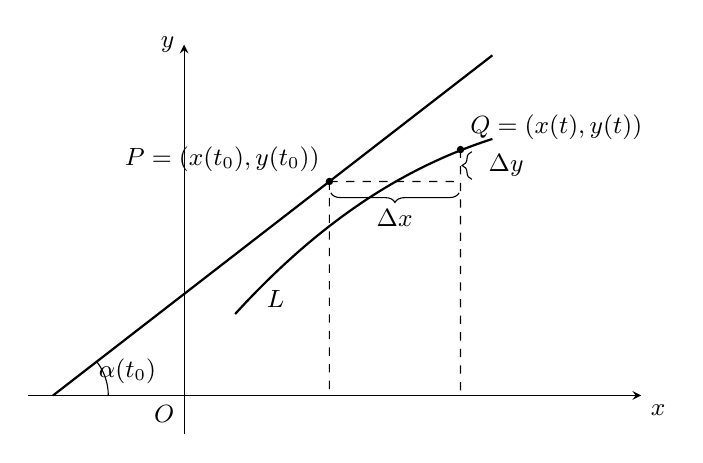
\begin{tikzpicture}[scale=0.9,>=stealth,font=\small]
  \draw[->] (-2.20,0) -- (6.45,0) node[below right] {$x$};
  \draw[->] (0,-0.55) -- (0,4.95) node[left] {$y$};
  \node[below left] at (0,0) {$O$};
  % 曲线 L
  \draw[thick] (0.72,1.15) .. controls (2.00,2.55) and (3.20,3.25) .. (4.35,3.62);
  \node[below left] at (1.55,1.62) {$L$};
  % 切线
  \draw[thick] (-1.85,0) -- (4.35,4.80);
  % P, Q
  \coordinate (P) at (2.05,3.02);
  \coordinate (Q) at (3.90,3.47);
  \fill (P) circle (1.5pt);
  \fill (Q) circle (1.5pt);
  \node[above left] at (P) {$P = (x(t_0), y(t_0))$};
  \node[above right] at (Q) {$Q = (x(t), y(t))$};
  % 虚线
  \draw[dashed] (P) -- (3.90,3.02);
  \draw[dashed] (P) -- (2.05,0);
  \draw[dashed] (Q) -- (3.90,0);
  % Delta x / Delta y
  \draw[decorate,decoration={brace,amplitude=3.5pt,mirror}] (2.07,2.86) -- (3.88,2.86);
  \node at (2.97,2.50) {$\Delta x$};
  \draw[decorate,decoration={brace,amplitude=3.5pt}] (4.06,3.05) -- (4.06,3.44);
  \node[right] at (4.16,3.24) {$\Delta y$};
  % 角 alpha(t0)
  \draw (-1.85,0) ++(0.78,0) arc (0:37.7:0.78);
  \node at (-0.80,0.34) {$\alpha(t_0)$};
\end{tikzpicture}
\caption{}\label{fig:3.2.1}
\end{figure}

如果 $x = x(t)$ 具有反函数 $t = t(x)$, 则
\[
y = y(t) = y(t(x)).
\]
这时只要 $x(t)$, $y(t)$ 可导, $x'(t) \neq 0$ (因而当 $\Delta x \to 0$ 时, 也有 $\Delta t \to 0$ 与 $\Delta y \to 0$), 就有
\[
\frac{\mathrm{d}y}{\mathrm{d}x} = \frac{\mathrm{d}y}{\mathrm{d}t}\cdot\frac{\mathrm{d}t}{\mathrm{d}x} = \frac{\mathrm{d}y}{\mathrm{d}t}\bigg/\frac{\mathrm{d}x}{\mathrm{d}t} = \frac{y'(t)}{x'(t)},\ \text{或}\ y'_{x} = \frac{y'_{t}}{x'_{t}}.
\]
如果 $x(t)$, $y(t)$ 均 2 阶可导, 则
\[
\begin{aligned}
\frac{\mathrm{d}^{2}y}{\mathrm{d}x^{2}} &= \frac{\mathrm{d}}{\mathrm{d}x}\left(\frac{\mathrm{d}y}{\mathrm{d}x}\right) = \frac{\left(\frac{y'(t)}{x'(t)}\right)'}{x'(t)} = \frac{y''(t)x'(t) - y'(t)x''(t)}{x'(t)[x'(t)]^{2}}\\
&= \frac{x'(t)y''(t) - y'(t)x''(t)}{[x'(t)]^{3}}.
\end{aligned}
\]
当曲线 $L$ 由极坐标方程 $\rho = \rho(\theta)$ 表示, 则可用极角 $\theta$ 作为参数, 即
\[
(x, y) = (\rho(\theta)\cos\theta, \rho(\theta)\sin\theta).
\]
如果 $\rho$ 可导, 则曲线 $\rho = \rho(\theta)$ 上点 $M(\rho, \theta)$ 处切线 $MT$ 与极轴 $Ox$ 轴的夹角 $\alpha$ 的正切(即切线斜率)为
\[
\begin{aligned}
\tan\alpha &= \frac{\mathrm{d}y}{\mathrm{d}x} = \frac{y'(\theta)}{x'(\theta)} = \frac{(\rho(\theta)\sin\theta)'}{(\rho(\theta)\cos\theta)'}\\
&= \frac{\rho'(\theta)\sin\theta + \rho(\theta)\cos\theta}{\rho'(\theta)\cos\theta - \rho(\theta)\sin\theta} = \frac{\rho'(\theta)\tan\theta + \rho(\theta)}{\rho'(\theta) - \rho(\theta)\tan\theta}.
\end{aligned}
\]
如图~\ref{fig:3.2.2} 所示, 过点 $M$ 的射线 $OH$ ($O$ 为极点, $Ox$ 为极轴) 与切线 $MT$ 的夹角 $\varphi$ 的正切为
\[
\begin{aligned}
\tan\varphi &= \tan(\alpha - \theta) = \frac{\tan\alpha - \tan\theta}{1 + \tan\alpha\tan\theta}\\
&= \frac{\frac{\rho'(\theta)\tan\theta + \rho(\theta)}{\rho'(\theta) - \rho(\theta)\tan\theta} - \tan\theta}{1 + \frac{\rho'(\theta)\tan\theta + \rho(\theta)}{\rho'(\theta) - \rho(\theta)\tan\theta}\tan\theta}\\
&= \frac{\rho'(\theta)\tan\theta + \rho(\theta) - \rho'(\theta)\tan\theta + \rho(\theta)\tan^{2}\theta}{\rho'(\theta) - \rho(\theta)\tan\theta + \rho'(\theta)\tan^{2}\theta + \rho(\theta)\tan\theta}\\
&= \frac{\rho(\theta)(1 + \tan^{2}\theta)}{\rho'(\theta)(1 + \tan^{2}\theta)} = \frac{\rho(\theta)}{\rho'(\theta)}.
\end{aligned}
\]

\begin{figure}[htbp]
\centering
\begin{tikzpicture}[scale=0.95,>=stealth,font=\small]
  \draw[->] (-1.05,0) -- (5.45,0) node[below right] {$x$};
  \node[below left] at (0,0) {$O$};
  % 射线 OH
  \draw[thick] (0,0) -- (5.00,3.29);
  \node[right] at (5.05,3.35) {$H$};
  % 角 theta
  \draw (0,0) ++(0.95,0) arc (0:33.3:0.95);
  \node at (0.98,0.30) {$\theta$};
  % 曲线
  \draw[thick] (1.86,1.02) .. controls (2.20,1.28) and (2.46,1.53) .. (2.507,1.647)
        .. controls (2.55,1.75) and (2.70,2.55) .. (2.86,3.30);
  % 切线 MT
  \draw[thick] (1.835,0) -- (3.86,4.96);
  \node[right] at (3.82,4.90) {$T$};
  % 点 M
  \fill (2.507,1.647) circle (1.6pt);
  \node[left] at (2.36,1.70) {$M$};
  % 角 alpha
  \draw (1.835,0) ++(0.65,0) arc (0:67.8:0.65);
  \node at (2.30,0.42) {$\alpha$};
  % 角 varphi
  \draw (2.507,1.647) ++(33.3:0.70) arc (33.3:67.8:0.70);
  \node at (3.11,2.38) {$\varphi$};
\end{tikzpicture}
\caption{}\label{fig:3.2.2}
\end{figure}

\begin{example}\label{ex:3.2.9}
证明: 对数螺线 $\rho = \mathrm{e}^{\frac{\theta}{2}}$ 上所有点的切线与向径的夹角 $\varphi$ 为常量.
\end{example}

\begin{proof}
因为
\[
\tan\varphi = \frac{\rho(\theta)}{\rho'(\theta)} = \frac{\mathrm{e}^{\frac{\theta}{2}}}{\frac{1}{2}\mathrm{e}^{\frac{\theta}{2}}} = 2,
\]
所以 $\varphi = \arctan 2$ 为常量.
\end{proof}

\begin{example}\label{ex:3.2.10}
求由上半椭圆的参数方程 $(x, y) = (a\cos t, b\sin t)$, $0 < t < \pi$ 所确定的函数 $y = y(x) = b\sqrt{1 - \frac{x^{2}}{a^{2}}}$ 的导数 $\frac{\mathrm{d}y}{\mathrm{d}x}$ 与 2 阶导数 $\frac{\mathrm{d}^{2}y}{\mathrm{d}x^{2}}$.
\end{example}

\begin{solution}
\[
\frac{\mathrm{d}y}{\mathrm{d}x} = \frac{\mathrm{d}y}{\mathrm{d}t}\bigg/\frac{\mathrm{d}x}{\mathrm{d}t} = \frac{b\cos t}{-a\sin t} = -\frac{b}{a}\cot t.
\]
\[
\frac{\mathrm{d}^{2}y}{\mathrm{d}x^{2}} = \frac{\mathrm{d}}{\mathrm{d}x}\left(\frac{\mathrm{d}y}{\mathrm{d}x}\right) = \frac{-\frac{b}{a}(\cot t)'}{-a\sin t} = \frac{-\frac{b}{a}(-\csc^{2}t)}{-a\sin t} = -\frac{b}{a^{2}\sin^{3}t}.
\]
或直接代入公式得到
\[
\begin{aligned}
\frac{\mathrm{d}^{2}y}{\mathrm{d}x^{2}} &= \frac{x'(t)y''(t) - y'(t)x''(t)}{[x'(t)]^{3}}\\
&= \frac{(-a\sin t)(-b\sin t) - (b\cos t)(-a\cos t)}{(-a\sin t)^{3}}\\
&= -\frac{b}{a^{2}\sin^{3}t}.
\end{aligned}
\]
请读者对 $y = b\sqrt{1 - \frac{x^{2}}{a^{2}}}$ 关于 $x$ 求 1 阶、2 阶导数来验证上述结果.
\end{solution}

\begin{example}\label{ex:3.2.11}
求由摆线参数方程 $(x, y) = (a(t - \sin t), a(1 - \cos t))$ 所确定的函数 $y = y(x)$ 的 2 阶导数.
\end{example}

\begin{solution}
\[
\frac{\mathrm{d}y}{\mathrm{d}x} = \frac{y'(t)}{x'(t)} = \frac{a\sin t}{a(1 - \cos t)} = \frac{2\sin\frac{t}{2}\cos\frac{t}{2}}{2\sin^{2}\frac{t}{2}} = \cot\frac{t}{2},
\]
\[
\frac{\mathrm{d}^{2}y}{\mathrm{d}x^{2}} = \frac{\mathrm{d}}{\mathrm{d}x}\left(\frac{\mathrm{d}y}{\mathrm{d}x}\right) = \frac{\left(\cot\frac{t}{2}\right)'}{a(1 - \cos t)} = \frac{-\frac{1}{2}\csc^{2}\frac{t}{2}}{2a\sin^{2}\frac{t}{2}} = -\frac{1}{4a}\csc^{4}\frac{t}{2}.
\]
\end{solution}

\begin{example}\label{ex:3.2.12}
设曲线参数方程为 $(x, y) = (1 - t^{2}, t - t^{2})$, 求它在 $t = 1$ 处的切线方程与法线方程.
\end{example}

\begin{solution}
因为
\[
\frac{\mathrm{d}y}{\mathrm{d}x}\bigg|_{t=1} = \frac{y'_{t}}{x'_{t}}\bigg|_{t=1} = \frac{1 - 2t}{-2t}\bigg|_{t=1} = \frac{1}{2},
\]
故切线方程为 $y - 0 = \frac{1}{2}(x - 0)$, 即 $y = \frac{1}{2}x$; 法线方程为 $y - 0 = -2(x - 0)$, 即 $y = -2x$.
\end{solution}

\begin{remark}\label{rem:3.2.2}
加速度是位移 $x(t)$ 对时间 $t$ 的 2 阶导数, 这是高阶导数在物理中的应用. 在古典微分几何中, 考虑 2 阶连续可导的正则曲线 $(x(t), y(t))$, 所谓正则指的是 $(x'(t))^{2} + (y'(t))^{2} \neq 0$, 从反映它弯曲程度的曲率公式
\[
\kappa(t) = \frac{x'(t)y''(t) - x''(t)y'(t)}{\left[(x'(t))^{2} + (y'(t))^{2}\right]^{3/2}},
\]
可看出 2 阶导数在几何中的重要应用. 在 3.6 节, 我们还可用 2 阶导数来刻画曲线的凹凸性与拐点以及判断函数的驻点(即 1 阶导数为 0 的点)是否为极值点, 是极大值点还是极小值点.
\end{remark}

\begin{exblock}{练习题 3.2}
  \item 求 $y$ 关于 $x$ 的 2 阶导数 $y''$.
  \begin{enumerate}[label=(\arabic*)]
    \item $y = \mathrm{e}^{-x^{2}}$;
    \item $y = x^{2}a^{x}$ ($a > 0$);
    \item $y = \ln\sin x$;
    \item $y = (1 + x^{2})\arctan x$;
    \item $y = \frac{\arcsin x}{\sqrt{1 - x^{2}}}$;
    \item $y = x\ln x$.
  \end{enumerate}

  \item 
  \begin{enumerate}[label=(\arabic*)]
    \item 设 $f(x) = \mathrm{e}^{2x-1}$, 求 $f''(0)$;
    \item 设 $f(x) = \arctan x$, 求 $f''(1)$;
    \item 设 $f(x) = \sin^{2}x$, 求 $f''\left(\frac{\pi}{2}\right)$;
    \item 设 $f(x) = 3x^{3} + 4x^{2} - 5x - 9$, 求 $f''(1)$, $f'''(1)$, $f^{(4)}(1)$.
  \end{enumerate}

  \item 求下列高阶导数:
  \begin{enumerate}[label=(\arabic*)]
    \item $f(x) = \frac{1+x}{\sqrt{1-x}}$, 求 $f^{(10)}(x)$;
    \item $f(x) = \frac{x^{2}}{1-x}$, 求 $f^{(8)}(x)$;
    \item $f(x) = \mathrm{e}^{-x^{2}}$, 求 $f''(x)$;
    \item $f(x) = \ln(1+x)$, 求 $f^{(5)}(x)$;
    \item $f(x) = x^{3}\mathrm{e}^{x}$, 求 $f^{(10)}(x)$.
  \end{enumerate}

  \item 设函数 $f$ 在 $(-\infty, x_0]$ 上 2 阶可导,
  \[
  F(x) = \begin{cases}f(x), & x \leqslant x_0,\\ a(x-x_0)^{2} + b(x-x_0) + c, & x > x_0.\end{cases}
\]
  问: 当 $a$, $b$, $c$ 为何值时函数 $F$ 在 $\mathbb{R}$ 上有 2 阶导函数.

  \item 设 $f$ 为 2 阶可导函数, 求下列各函数的 2 阶导函数.
  \begin{enumerate}[label=(\arabic*)]
    \item $y = f(\ln x)$;
    \item $y = f(x^{n})$, $n \in \mathbb{N}$;
    \item $y = f(f(x))$.
  \end{enumerate}

  \item 设函数 $f$ 在点 $x = 1$ 处 2 阶可导, $f'(1) = 0$, $f''(1) = 0$. 证明: 在 $x = 1$ 处有
  \[
  \frac{\mathrm{d}}{\mathrm{d}x}f(x^{2}) = \frac{\mathrm{d}^{2}}{\mathrm{d}x^{2}}f^{2}(x).
\]

  \item 求下列函数的 $n$ 阶导数:
  \begin{enumerate}[label=(\arabic*)]
    \item $y = \ln x$;
    \item $y = \frac{\ln x}{x}$;
    \item $y = \frac{1}{x(1-x)}$;
    \item $f(x) = \frac{x^{n}}{1-x}$;
    \item $v = \mathrm{e}^{ax}\sin bx$ ($a$, $b$ 均为实数).
  \end{enumerate}

  \item 设 $y = \frac{ax+b}{cx+d}$. 证明:
  \[
  y^{(n)}(x) = (-1)^{n+1}\frac{n!\,c^{n-1}}{(cx+d)^{n+1}}\begin{vmatrix}a & b\\ c & d\end{vmatrix}.
\]

  \item 证明: 函数
  \[
  f(x) = \begin{cases}\mathrm{e}^{-\frac{1}{x^{2}}}, & x \neq 0,\\ 0, & x = 0\end{cases}
\]
  在 $x = 0$ 处 $n$ 阶可导, 且 $f^{(n)}(0) = 0$, 其中 $n \in \mathbb{N}$.

  \item 求由下列参数方程所确定的函数的 2 阶导数 $\frac{\mathrm{d}^{2}y}{\mathrm{d}x^{2}}$:
  \begin{enumerate}[label=(\arabic*)]
    \item $\begin{cases}x = a\cos^{3}t,\\ y = a\sin^{3}t;\end{cases}$
    \item $\begin{cases}x = \mathrm{e}^{t}\cos t,\\ y = \mathrm{e}^{t}\sin t;\end{cases}$
    \item $\begin{cases}x = \cos^{4}t,\\ y = \sin^{4}t;\end{cases}$
    \item $\begin{cases}x = \frac{t}{1+t},\\ y = \frac{1-t}{1+t}.\end{cases}$
  \end{enumerate}

  \item 证明: 原点到曲线
  \[
  \begin{cases}x = a(\cos t + t\sin t),\\ y = a(\sin t - t\cos t)\end{cases}
\]
  上任一点的法线的距离等于 $a$.

  \item 证明: 圆 $r = 2a\sin\theta$ ($a > 0$) 上任一点的切线与向径的夹角等于向径的极角.

  \item 求心形(脏)线 $r = a(1 + \cos\theta)$ 的切线与切点向径之间的夹角.
\end{exblock}

\begin{exblock}{思考题 3.2}
  \item 设 $m$, $n \in \mathbb{N}$. 证明:
  \[
  \sum_{k=0}^{n}(-1)^{k}\mathrm{C}_{n}^{k}k^{m} = \begin{cases}0, & m \leqslant n-1,\\ (-1)^{n}n!, & m = n.\end{cases}
\]

  \item 设 $u$, $v$, $w$ 都为 $t$ 的可导函数. 试给出 $(uvw)^{(n)}$ 的 Leibniz 公式, 这里 $n \in \mathbb{N}$.

  \item 设 $y = x^{n-1}\mathrm{e}^{\frac{1}{x}}$. 证明:
  \[
  y^{(n)} = \frac{(-1)^{n}}{x^{n+1}}\mathrm{e}^{\frac{1}{x}}.
\]

  \item 设 $y = \arctan x$. 证明:
  \[
  y^{(n)} = \frac{P_{n-1}(x)}{(1+x^{2})^{n}},
\]
  其中 $P_{n-1}$ 为最高次项系数是 $(-1)^{n-1}n!$ 的 $n-1$ 次多项式.

  \item 设 $f(x) = x^{n}\ln x$, $n \in \mathbb{N}$, 求极限
  \[
  \lim_{n\to+\infty}\frac{f^{(n)}\left(\frac{1}{n}\right)}{n!}.
\]

  \item 证明: 在 $\mathbb{R}$ 上不存在可导函数 $f$ 满足 $f^{2}(x) = -x^{3} + x^{2} + 1$.

  \item 证明: 在 $\mathbb{R}$ 上不存在可导函数 $f$ 满足 $f^{2}(x) = x^{2} - 3x + 3$.

  \item 求 $\left(\mathrm{e}^{x}\cos x\right)^{(n)}$ 与 $\left(\mathrm{e}^{x}\sin x\right)^{(n)}$.

  \item 设 $y = (1 + \sqrt{x})^{2n+2}$, $n \in \mathbb{N}$, 求 $y^{(n)}(1)$.

  \item 设多项式 $p$ 只有实零点, 证明: $(p'(x))^{2} \geqslant p(x)p''(x)$ 对一切 $x \in \mathbb{R}$ 成立.

  \item 设 $y = \arctan x$.
  \begin{enumerate}[label=(\arabic*)]
    \item 证明它满足方程 $(1+x^{2})y'' + 2xy' = 0$;
    \item 求 $y^{(n)}(0)$.
  \end{enumerate}

  \item 设 $f(x) = \arctan x$. 证明:
  \[
  f^{(n)}(x) = (n-1)!\cos^{n}f(x)\cdot\sin\left(f(x) + \frac{n\pi}{2}\right).
\]
\end{exblock}
